\begin{frame}{Sampling $z'$ from vMF}
  \begin{algorithm}[H]
    \caption{Overview of the sampling method from $vMF(\mu, \kappa)$}\label{alg:overviewsampling}
    \begin{algorithmic}[1]
      \STATE Sample $z \sim q(z| e_1, \kappa)$ where $e_1 = (1, 0, \dots, 0)$
      \STATE Compute Householder reflection $U(\mu)$ so that $U(\mu) e_1 = \mu$
      \RETURN $z' = U(\mu) z$
    \end{algorithmic}
    \end{algorithm}
  \end{frame}

  \begin{frame}{Sampling $z$ from vMF}
    \begin{algorithm}[H]
      \caption{Overview of the sampling method from $vMF(\mu, \kappa)$}\label{alg:overviewsampling2}
      \begin{algorithmic}[1]
        \STATE Sample $z \sim q(z| e_1, \kappa)$ where $e_1 = (1, 0, \dots, 0)$
        \textcolor{red}{
          \STATE Sample $w \in \mathbb{R} \sim g(w |\kappa)$ by acceptance rejection sampling
          \STATE Sample $v \in \mathbb{R}^{d-1} \sim \mathcal{U}(S^{d-2})$ (uniform on the hypersphere $S^{d-2}$ independent of $w$)
          \STATE $z \gets (w, \sqrt{1 - w^2}v^T)^T$
        }
        \textcolor{gray}{
        \STATE Compute Householder reflection $U(\mu)$ so that $U(\mu) e_1 = \mu$
        \RETURN $z' = U(\mu) z \sim q(z' | \mu, \kappa)$}
      \end{algorithmic}
      \end{algorithm}
    \end{frame}
  
\begin{frame}{Sampling $w$ from $g(w|\kappa, \theta)$}
  \centering
  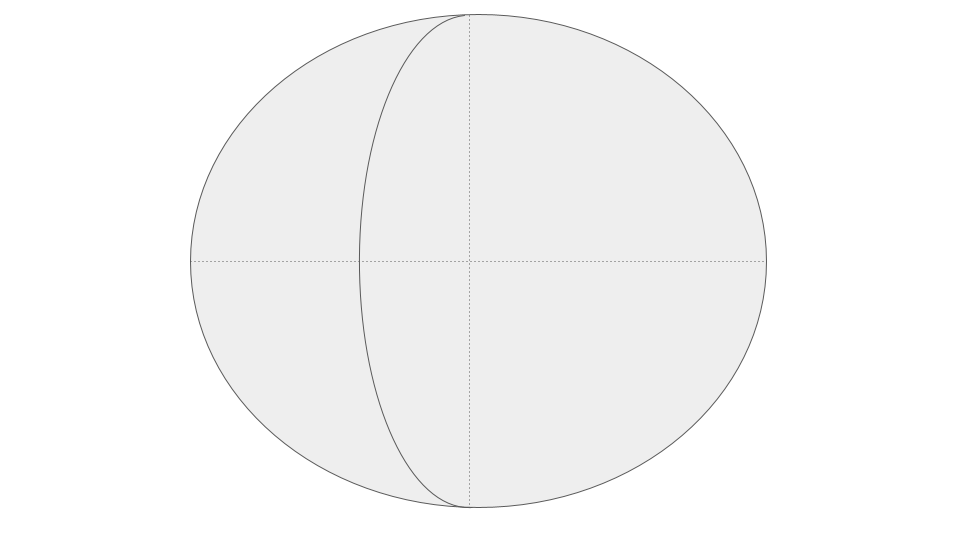
\includegraphics[width=\textwidth]{figures/illustration_sampling_1.png}
  $S^{2}$ : unit sphere in $\mathbb{R}^{3}$
\end{frame}

\begin{frame}{Sampling $w$ from $g(w|\kappa, \theta)$}
  \centering
  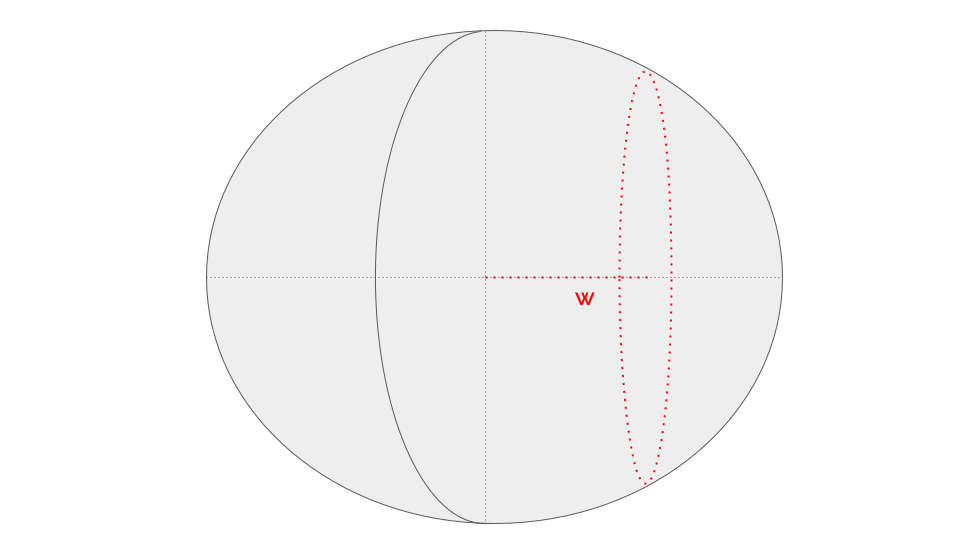
\includegraphics[width=\textwidth]{figures/illustration_sampling_2.png}  
  Sample $w \in \mathbb{R} \sim g(w |\kappa, d)$ by acceptance rejection sampling
\end{frame}

\begin{frame}{Sampling $w$ from $g(w|\kappa)$}
  \begin{itemize}
    \item[$\blacksquare$] Generale case
    \begin{itemize}
      \item Sample target distribution $w \in \mathbb{R} \sim g(w |\kappa)$ by sampling a proposal $w_{prop}$ of known density $r(w|\kappa)$
      \item Perform backpropagation by reparameterizing $r(w| \kappa)$ so that the sampling is independent of the parameters
      \item Note that $r$ is not explicitly given in the article
    \end{itemize}
  \end{itemize}
  \vfill
  \centering
  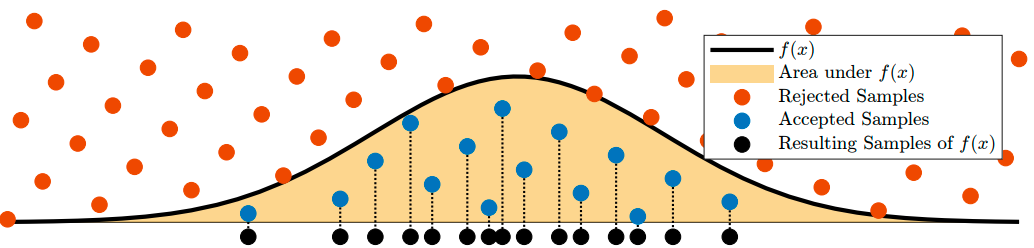
\includegraphics[height=.3\textheight]{figures/sampling_meth_illustration.png}
  \tiny{Illustration from \cite{frisch_rejection_2022}}
\end{frame}

\begin{frame}{Sampling $w$ from $g(w|\kappa)$}
  \begin{itemize}
    \item[$\blacksquare$] Case $d=3$ : faster to use inverse transformation method
    \begin{itemize}
      \item The vMF distribution explicity writes : $$ f_{vMF}(z) = \frac{\kappa}{4\pi\ sinh(\kappa)} exp(\kappa\mu^T z)  $$
      \item $(w, \sqrt{1 - w^2}v^T)^T \sim vMF(e_1, \kappa)$ where $v \sim \mathcal{S}^2$ and $w\in [-1, 1]$ has density $$ f_{W}(w) = \frac{\kappa}{2\ sinh(\kappa)} exp(\kappa w) $$
      \item We compute its cumulative distribution function $F_W(w)$ and its inverse  $$ F^{-1}_W (u) = \frac{1}{\kappa} ln(exp(-\kappa) + 2\ sinh(\kappa)u ) $$
      \item As $ sinh(\kappa) $ is numerically instable, we rewrites $$ F_W^{-1}(u) = 1 + \frac{1}{\kappa} ln(u + (1-u)exp(-2\kappa)) $$
    \end{itemize}
  \end{itemize}
\end{frame}

\begin{frame}{Sampling $v$ from $\mathcal{U}(S^{d-2})$}
  \centering
  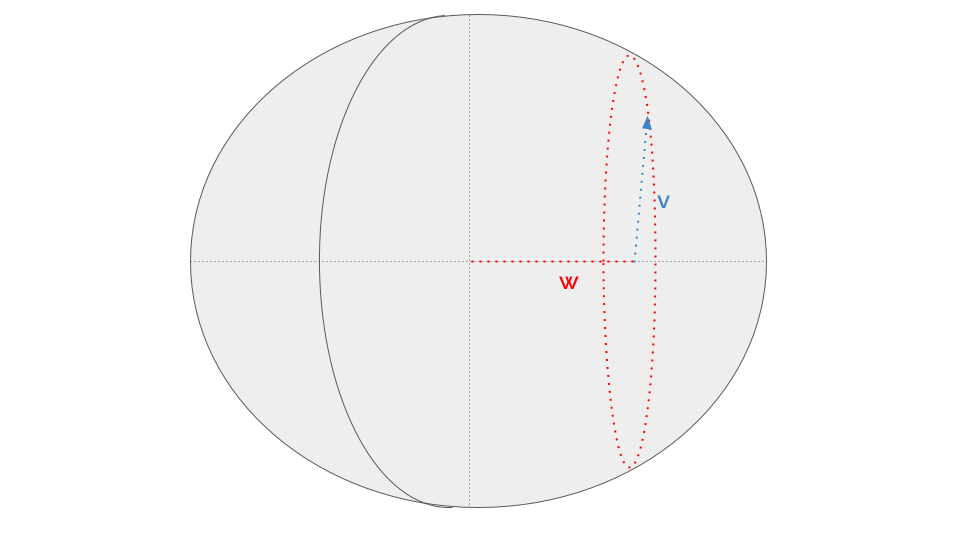
\includegraphics[width=\textwidth]{figures/illustration_sampling_3.png}
  \textcolor{blue}{Sample $v \in \mathbb{R}^{d-1} \sim \mathcal{U}(S^{d-2})$}
\end{frame}

\begin{frame}{Sampling $v$ from $\mathcal{U}(S^{d-2})$}
  \begin{itemize}
    \item $\mathcal{N}(0, I_{d-1})$ is rotationally symmetric around the origin
    \item $f_{Y_1, \dots, Y_{d-1}} = \frac{1}{\sqrt{2\pi}^{d-1}} exp(- (Y_1^2 + \dots + Y_{d-1}^2)/2) = \frac{1}{\sqrt{2\pi}^{d-1}}exp(-1^2/2) $ which is constant in all of the angular variables.
  \end{itemize}
  \vfill
  \begin{algorithm}[H]
    \caption{Sampling $v$ from $\mathcal{U}(S^{d-2})$}
  \begin{algorithmic}[1]
    \STATE Generate $d-1$ \textit{iid} variables $(X_i)$ from $\mathcal{N}(0, 1)$
    \STATE $Y_i \gets \frac{X_i}{\sqrt{X_1^1 + \dots + X_{d-1}^2}}$
    \RETURN $(Y_i)_{i=1, \dots, d-1} \sim \mathcal{U}(S^{d-2})$  
  \end{algorithmic}
  \end{algorithm}
\end{frame}

\begin{frame}{Sampling $z$ from $q(z|e_1, \kappa)$}
  \centering
  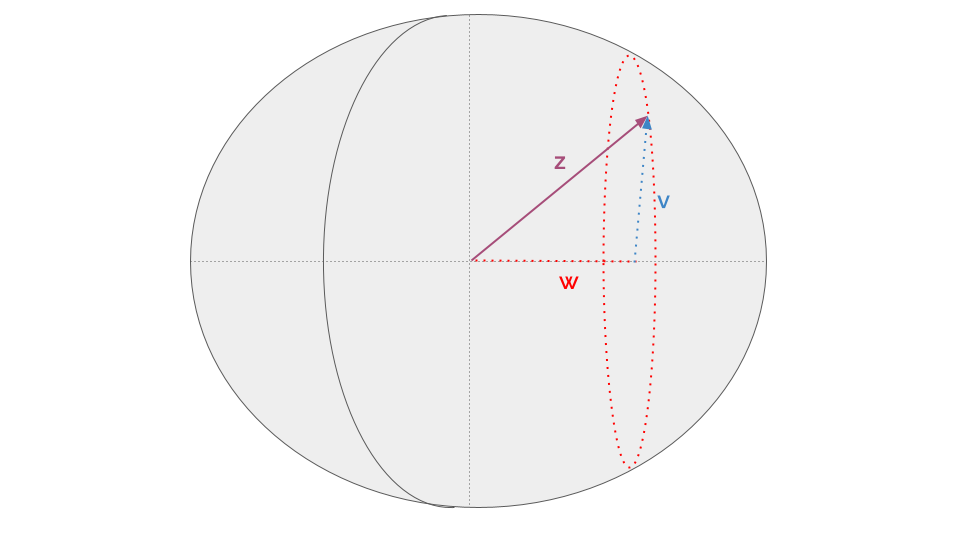
\includegraphics[width=\textwidth]{figures/illustration_sampling_4.png}
  \textcolor{magenta}{$z = (w, \sqrt{1 - w^2}v^T)^T$}
\end{frame}

\begin{frame}{Transform $z$}
  \begin{algorithm}[H]
    \caption{Overview of the sampling method from $vMF(\mu, \kappa)$}\label{alg:overviewsampling3}
    \begin{algorithmic}[1]
      \REQUIRE $\mu \in \mathbb{R}^d$, $\kappa \in \mathbb{R}_+$
      \textcolor{gray}{ \STATE Sample $z \sim q(z| e_1, \kappa)$ where $e_1 = (1, 0, \dots, 0)$ }
      \STATE Compute Householder reflection $U(\mu)$ so that $U(\mu) e_1 = \mu$
      \textcolor{red}{
      \STATE $u \gets Normalize(e_1 - \mu)$ 
      \STATE $U \gets I - 2uu^T$}
     \textcolor{red}{\RETURN $z' = U(\mu) z$}
    \end{algorithmic}
    \end{algorithm}
\end{frame}